\documentclass[twocolumn, a4paper]{ieicejsp}
%\documentclass[twocolumn,a4paper]{jsarticle}
\usepackage[hang,bf,labelsep=space,figurename=図, tablename=表]{caption}
% \usepackage{newenum}
\usepackage{epsfig}
% \usepackage{comment}
% \usepackage{setspace}
\usepackage{multirow}
\usepackage{verbatim}
\usepackage{subfigure}
\usepackage{fancyvrb}
\usepackage{subfig}
\usepackage{subfigmat}
\usepackage[dvipdfmx]{}
%\usepackage{mediabb}
%\usepackage[dvipdfmx]{}
% \usepackage{sty/moreverb}
% \usepackage{color}
%プログラムソースコード

% \newcommand{\LISTFSIZE}{small}
\newcommand{\LISTBASELINE}{0.90} % 図の行間
\newcommand{\verbg}{\underline{x0}}
\newcommand{\verbgt}{\underline{t0}}
\renewcommand{\baselinestretch}{1.02}
% \usepackage{listings,xcolor}

\setlength{\topmargin}{0pt}
\setlength{\textheight}{248mm}

\makeatletter
\def\abstract#1{\long\def\@abstract{#1}}
\def\@abstract{}
\let\@oldmaketitle=\@maketitle
\def\@maketitle{
    \vskip -3zh
    \vspace{-2mm}
\begin{flushright}
卒業研究審査会 2020年2月21日
\end{flushright}
% \vspace{3mm}
\begin{center}
\LARGE
\bf 機械学習を用いたファズデータの \\[-0.3em] チェックサム及びハッシュ値の推定

\medskip
\large 石浦研究室~~27016627~~藤本 高史
\end{center}
    \vskip 1.5em}
\makeatother
\setlength\intextsep{0pt}
\setlength\textfloatsep{-10pt}


\begin{document}
\maketitle
\section{はじめに}

ソフトウェアの脆弱性は社会的に深刻な問題をもたらしており,
リリース前に十分なテストを行うことが重要な課題になっている.
ファジングは, 自動的に生成した大量の入力データによって対象プログラム
をテストする, セキュリティなどの脆弱性の検出手法である.
変異ベース手法は実装が容易で, 汎用性も高いが,
入力データの棄却率が高く, 効率的にファジングを行えていないことが課題となる.
%入力データ作成に用いられる変異ベース手法は,
%チェックサムにより入力データの棄却率が高く, 効率的にファジング行えていないことがあげられる.
この課題に対し, 文献\cite{namba}はLSTMを用いて入力データに対するチェックサムの推定を行い, 68 \%の正答率となった.
しかし, 8 byteのデータに対するチェックサムのみしか対応していないため, 汎用性に欠ける課題がある.
%ファジングには, 仕様書などを使い一から入力データを生成する生成ベース手法と,
%既存のファイルの一部を書き換えて新たな入力データを生成する変異ベース手法が存在する.

本研究では, 8 byte以上のデータに対するチェックサム及び様々なハッシュ値の推定を行う.

%\vspace{-3mm}

%\section{チェックサムおよびハッシュ値によるデータの検査}
\section{ニューラルネットワークによるチェックサムの推定}

文献\cite{namba}はニューラルネットワークを用いて, 8 byteの入力データに対するチェックサムの推定を行っている.
正規データからデータとチェックサムの集合を抽出し, ニューラルネットワークに学習させる.
学習済ニューラルネットワークで変異データからチェックサムを推定し, 更新する.
学習の流れを, 図\ref{namba}に示す.
初めに, 文字列とその文字列に対するチェックサムのデータを用意する.
次に, そのデータをニューラルネットワークへ入力をし, 学習を行う.
そして, 学習済ニューラルネットワークに対して, 文字列を入力することにより, チェックサム及びハッシュ値を推定する.
最後に, 推定したチェックサムを, 文字列の末端に付与する.
よって, 正当な入力データとして扱われる.

\vspace{1mm}
\begin{figure}[htbp]
%\begin{minipage}{0.5\hsize}
 \begin{center}
  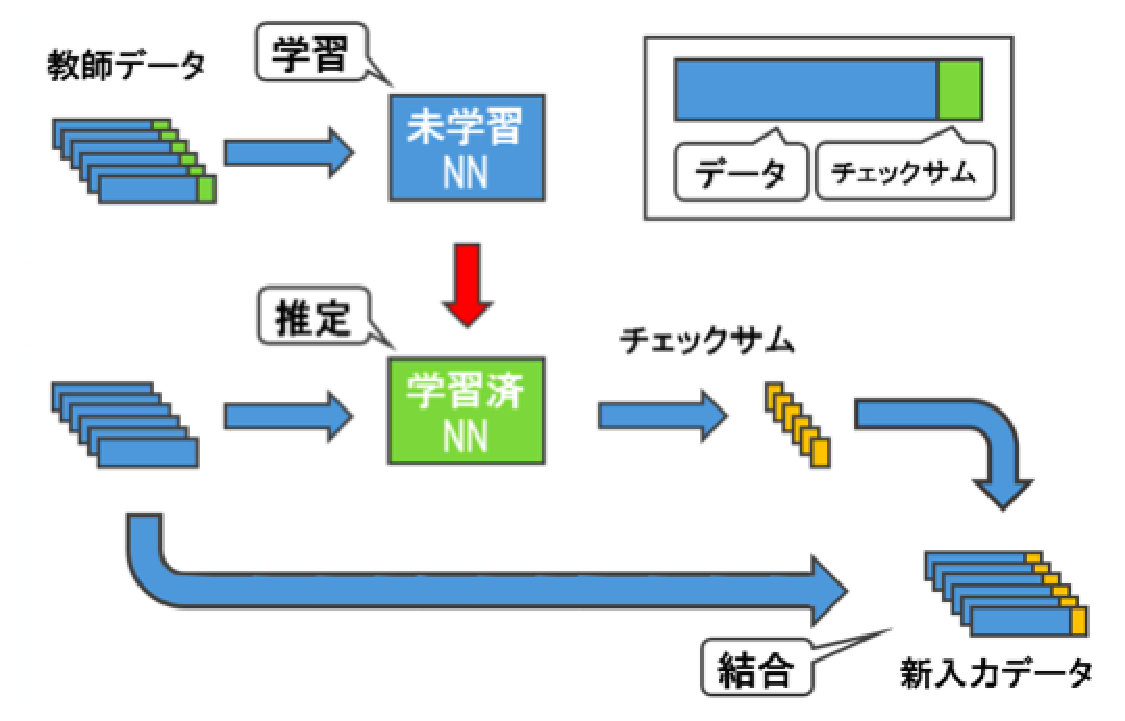
\includegraphics[width=60mm]{namba_gakusyu.eps}
  \caption{学習の流れ}
   \label{namba}
 \end{center}
%\end{minipage}
\end{figure}

\vspace{1mm}
%チェックサムは, 誤り検出符号の一方式である
%主に通信データやファイル内容などの検証に使用されており, 計算方法はデータ列の和を求め, 256の剰余をとる.

%ハッシュ値は, 誤り検出符号の一方式である.
%文字列からハッシュ関数を通して, 特定のルールにしたがって計算し, 固定長の規則性のない文字列が出力される.
%ハッシュ値はファイル同一性の確認に用いられており, 特徴としてハッシュ値から入力値の推測が不可能であり,
%同じハッシュ値が出力されることがないため, 暗号やパスワードにも利用される.
%入力データは論理的にいくつかのチャンクに分割されており,
%各データのチェックサムまたはハッシュ値が後ろに付加される.
%入力データは論理的にいくつかの``チャンク''に分割されており,
%各データのハッシュ値が後ろに付加される.
%誤り訂正符号としては, データの総和を定数で割った剰余(checksum), CRC, MD5などを想定する.

%変異ベース手法のファジングで, 入力データの一部を変異させる際, 変異させた箇所のチェックサムまたはハッシュ値が正しい値に修正できなければ,
%入力データは対象プログラムにとって不正なものとして棄却されてしまう.
%そのため, 本研究では変異させた箇所のチェックサムまたはハッシュ値を推定することにより, 不正な入力データとして
%棄却されるのを防ぎ, 効率的にファジングを行うことが可能になる.


\section{機械学習によるチェックサム及びハッシュ値の推定}

本研究では, 8 byte以上のデータに対するチェックサム及び様々なハッシュ値の推定を行う.
データとチェックサムおよびハッシュ値の位置とハッシュ関数の種類は既知であることを前提とする.
%固定長の入力データでどのバイト数までのデータならチェックサムを推定することが可能か調査を行う.
固定長ではなく, 可変長の入力データで学習を行う.
学習に関しては, Encoder・Decoderモデル\cite{seq2seq}を利用したニューラルネットワークを構成して学習する.
この時, 各ノード数などのパラメータは, どのような入力及び出力を行うかによって最適な値が異なるため, 実験を繰り返して最適な値を見つける.
%ハッシュ値の推定の方法はチェックサムと同様に行う.
また, 推定する値によって計算方法は変わってくるため, 各々の値に対応した機械学習を行う.
%チェックサムとハッシュ値の学習は2 パターン行う.
%1 つ目は正規データからデータとチェックサムまたはハッシュ値の集合を抽出し, ニューラルネットワークに学習させる.
%学習済ニューラルネットワークで変異データからチェックサムまたはハッシュ値を推定し, 更新する.
%ハッシュ値変更前と変更後での通過率の比較を, ハッシュ値検査が採用されているソフトウェアで実施する.
%2 つ目は変異データの入力結果からデータとチェックサムまたはハッシュ値と対応の正否値を用意し, 学習させる.
%学習の後にデータとチェックサムまたはハッシュ値から対応を推定し, 対応していると判定されたデータのみ選抜する.
%なお, ハッシュ値のデータの位置は既知とする.
%データとハッシュ値の抽出は既に終えているものとする.
%また, ハッシュ値の機械学習のみに焦点をあてる.
%既存の正当な入力からデータとハッシュ値対の集合を抽出し, ニューラルネットワークに学習させる.
%変異させたデータからハッシュ値を学習済ニューラルネットワークで推定し, これに更新する.
%今回はハッシュ値の機械学習のみに焦点をあてる.
% \vspace{3mm}
%\begin{figure}[h]
%  \begin{center}
%    \begin{tabular}{ccc}
%            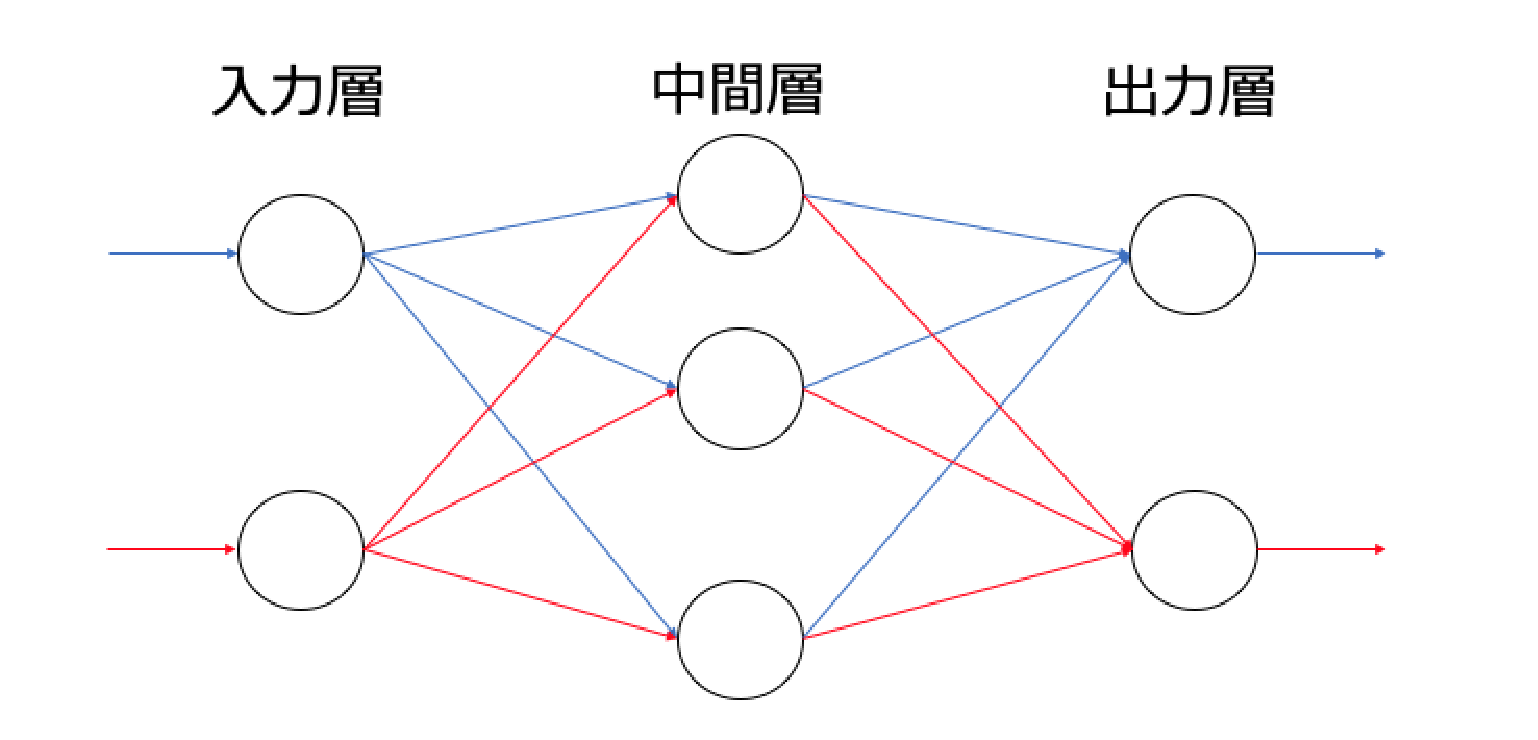
\includegraphics[width=7.0cm]{NN.eps}
%     \end{tabular}
%    \vspace{1mm}
%    \caption{\small 実験に用いたニューラルネットワークの構成}
%    \label{fig::nn}
%  \end{center}
%\end{figure}
% \vspace{2mm}
%\smallskip
%\vspace{-2mm}
\section{実験}

機械学習を用いて8 byte以上のランダム文字列と英文に対するチェックサム及びハッシュ値を推定する実験を行った.
提案手法をKerasを用いてPythonで実装し, 機械学習を実行した.
総データ数は10 $\sim$ 20 万文書である.
ランダム文字列は1 $\sim$ 64 byteの可変長の入力データである.
英文は文字列は2 $\sim$ 48 byteの可変長の入力データである.
学習させる文字列の長さ及びデータ数は, 推定する値によって異なる.
推定する値として, チェックサム, CRC16 \cite{crc}, CRC32 \cite{crc}, MD5 \cite{md5}, SHA1 \cite{sha1} で実験を行った.

学習時に得られた正答率と学習済ニューラルネットワークを用いて得られた正答率を, 表\ref{seitouritu}に示す.
Train Random, Train Englishは, 学習時に得られた正答率である.
Random, Englishが学習済ニューラルネットワークを使用した時に得られた正答率である.
学習時に得られた正答率と学習済ニューラルネットワークを使用して得られた正答率を比較すると, 必ずしも正答率が一致しないことがわかった.
特に, ランダム文字列の方が正答率が高かったり, 英文の方が正答率が高かったりなど, ばらつきが見られた.
%しかし, ランダムで当てる確率より遥かに高い精度が得られたことに変わりはない.
%\vspace{1mm}
%誤差は各データの正解値と推測値の誤差の平均であり, 的中率は各データの正解値と推測値が一致した割合である.
%1 回目ではテストデータの平均誤差が5.1648まで大きかったが, 20000 回目では0.6941 まで低下している.
%また, テストデータの的中率は0.0012 から0.6744 まで上昇している.
%教師データと値を比較しても, 誤差が小さく, 過学習が行われている可能性は低いと考えられるため, 信頼性は高いと思われる.
%変異ベース手法で生成された入力データの通過率が約10$\sim$15\% しかないため,
%このニューラルネットワークの学習精度は非常に良いと思われる.
%よって, 過学習が起こっており, 現段階では何も推定を行えていない状況である.
%そのため, ニューラルネットワークの構築やノード数を変更したりなどの様々なアプローチを試す必要性が懸念される.

%\vspace{3mm}
%\begin{table}[!h]
%  \begin{minipage}{0.9\linewidth}
%  \begin{center}
%  \centering
%  \caption{英文}
%  \begin{footnotesize}
%  \begin{tabular}{|r|r|r|r|r|}
%  \hline
%     & 学習データ & テストデータ & 学習誤差 & 推定誤差    \\ \hline 
%  チェックサム   & 72 \% & 72 \% & 0.66  & 0.66    \\ \hline
%  CRC16   & 57\% & 57\% & 0.57 & 0.57   \\ \hline
%  CRC32   & 53\% & 53\% & 0.65 & 0.65  \\ \hline
%  MD5  & 15\% & 15\% & 2.5  & 2.5    \\ \hline
%  SHA1    & 5\% & 5\% & 2.9  & 2.9    \\ \hline
%  \end{tabular}\label{english}
%  \end{footnotesize}
%  \end{center}
%  \end{minipage}
%  \end{table}


\vspace{6mm}
\begin{table}[!h]
\begin{minipage}{0.9\linewidth}
 \begin{center}
 \centering
 \caption{チェックサム及びハッシュ値の正答率}
  \begin{footnotesize}
  \begin{tabular}{|r|r|r|r|r|}
  \hline
     & Train Random & Train English & Random & English    \\ \hline
  cksum   & 52\% & 50\% & 20\% & 51\%   \\ \hline
  CRC16   & 53\% & 47\% & 9\% & 9\%   \\ \hline
  CRC32   & 54\% & 50\% & 12\% & 4\%   \\ \hline
  MD5  & 11\% & 11\% & 12\%  & 2\%    \\ \hline
  SHA1    & 14\% & 19\% & 5\%  & 11\%    \\ \hline
  \end{tabular}\label{seitouritu}
  \end{footnotesize}
  \end{center}
  \end{minipage}
\end{table}

%\vspace{4mm}
%\begin{table}[!h]
% \begin{tabular}{c}
%  \begin{minipage}{0.45\linewidth}
%  \centering
%  \caption{英文}
%  \begin{footnotesize}
%   \begin{tabular}{|r|r|}
%    \hline
%     &   学習精度 \\ \hline
%    チェックサム & 50.8 \%    \\ \hline
%    CRC16  & 9.08 \%    \\ \hline
%    CRC32  & 4.17 \%    \\ \hline
%    MD5  & 2.53 \%    \\ \hline
%    SHA1  & 10.75 \%    \\ \hline
%   \end{tabular}
%  \end{footnotesize}
%  \label{english}
%  \end{minipage}

%\hfill

%\vspace{4mm}
% \begin{minipage}{0.45\linewidth}
% \centering
% \caption{ランダム文字列}
%  \begin{footnotesize}
%  \begin{tabular}[t]{|r|r|r|}
%    \hline
%    &   学習精度 \\ \hline
%   チェックサム & 20 \%    \\ \hline
%   CRC16  & 9.01 \%    \\ \hline
%   CRC32  & 11.9 \%    \\ \hline
%   MD5  & 12.07 \%    \\ \hline
%   SHA1  & 4.95 \%    \\ \hline
%  \end{tabular}
%  \end{footnotesize}
%  \label{random}
%  \end{minipage}
%  \end{tabular}
%\end{table}


%\vspace{-2mm}
\vspace{1mm}
\section{むすび}
%これまでに, データとハッシュ値の学習を行い, 推定が可能かのテストを行った.
%これまでに, コンパイラの最適化性能テストのためのプログラム生成の一手法を考案し, 実装, テストを行った.
%今後の課題はニューラルネットワークの構成の改善, 構成のアルゴリズムの比較, 実験評価である.
%その結果, ハッシュ値を学習できた.
本研究では, ランダム文字列と英文からチェックサム及びハッシュ値の推定を行い, チェックサム, CRC16, CRC32, MD5, SHA1 を高精度で推定することができた.
今後の課題は, 精度向上, 他のハッシュ値の推定, 固定長による推定評価, 実装評価である.

\begin{footnotesize}
  \begin{thebibliography}{15}
%    \vspace{0.5mm}
\bibitem{namba} 難波 学之:
``変異ベースファジングのためのチェックサムの機械学習,''
関西学院大学理工学部情報科学科卒業論文 (Mar. 2019).

\bibitem{seq2seq} Ilya Sutskever, Oriol Vinyals, and Quoc V Le:
``Sequence to sequence learning with neural networks,''
in \textit{Proc. Nueral Information Processing Systems}, pp. 3104–3112 (Sept. 2014).

\bibitem{crc} Andrew Tanenbaum, David Weatherroll 著, 水野忠則 訳:
  コンピュータネットワーク,
 日経BP(Sept.\ 2013).

 \bibitem{md5} IPUSIRON 著:
  暗号技術のすべて,
 翔泳社(Aug.\ 2017).

 \bibitem{sha1} 林 芳樹 著:
  暗号理論入門,
 丸善出版(Apr.\ 2012).
  \end{thebibliography}

\end{footnotesize}

\end{document}
